\documentclass[english, 11pt]{article}
\usepackage{../../notes}
\usepackage{lipsum}

%Global Course Variables
\newcommand{\myCourseCode}{University of Toronto}
\newcommand{\myCourseName}{Neural Networks for Machine Learning}
\newcommand{\myProf}{Geoffrey Hinton}
\newcommand{\myTerm}{Summer 2015}
\newcommand{\myLogo}{UofT-Crest-Wide.png}

%Headers
\lhead{\myCourseName}
\rhead{\fancyplain{}{\rightmark}} 

%Footers
\cfoot{\thepage}

\begin{document}
\titleHeader{\myCourseCode}{\myCourseName}{\myProf}{\myTerm}{\myLogo}

%Document information
\noindent\rule{1\columnwidth}{.5pt}
Contributors: Max Smith
\begin{center}
	Latest revision: \today
\end{center}
\toc
\abstr{Neural networks use learning algorithms that are inspired by our understanding of how the brain learns, but they are evaluated by how well they work for practical applications such as speech recognition, object recognition, image retrieval and the ability to recommend products that a user will like. As computers become more powerful, Neural Networks are gradually taking over from simpler Machine Learning methods. They are already at the heart of a new generation of speech recognition devices and they are beginning to outperform earlier systems for recognizing objects in images. The course will explain the new learning procedures that are responsible for these advances, including effective new proceduresr for learning multiple layers of non-linear features, and give you the skills and understanding required to apply these procedures in many other domains.}

%----------------------------
%Document Begins
%----------------------------

\section{Introduction}

\section{The Perceptron learning procedure}

\section{The backpropagation learning proccedure}

\section{Learning feature vectors for words}

\section{Object recognition with neural nets}
	\subsection{After calibration}
\img{.8}{sections/lec5/p.png}
\begin{itemize}
	\item Internal parameters $K$ are known
	\item $R, T$ are known - but these can only relate $C$ to the calibraiton rig.
	\item You can't estimate $P_i$ from the single image measurement of $p_i$ because it may be anywhere along the line in space.
	\item We also don't have any information in the image to tell us the scale of anything in the world.
\end{itemize}

\subsection{Recovering structure from a single view}
\begin{itemize}
	\item You can make assumptions to get relative sizes of objects in images
	\item Pick a reference plane in the scene
	\item Pick a reference direction (not parallel to the reference plane) in the scene
	\img{.8}{sections/lec5/ref.png}
	\subsubsection{Geometry}
	\img{.8}{sections/lec5/van.png}
	\item Under perspective projection, parallel lines in three-space project to convering lines in the image plane. The common point of intersection, perhaps at infinity, is called the \textbf{vanishing point}
	\begin{itemize}
		\item projection of a point at infinity (goes infinity far)
		\img{.8}{sections/lec5/vp.png}
		\item Any two parallel lines have the same vanishing point
		\item The ray from $C$ through $v$ point is parallel to the lines
		\item AN image may have more than one vanishing point
	\end{itemize}
	\item Two or more vanishing points from lines known to lie in a single 3D plane establish a \textbf{vanishing line}, which completely determines the orientation of the plane
	\img{.7}{sections/lec5/house.png}
\end{itemize}

\subsection{The Cross Ratio}
\img{.8}{sections/lec5/y.png}
\begin{itemize}
	\item $Y$ is desired height to measure
	\item Compute Y from image measurements
	\begin{itemize}
		\item You'll need more than vanishing points to compute this
	\end{itemize}
	\item \textbf{Projective Invariant}: something that does not change under projective transformations (including perspective projection)
	\img{.8}{sections/lec5/l.png}
	\item The \textbf{cross ratio} of 4 collinear points is projective invariant
	$$\frac{||P_3 - P_1||\cdot ||P_4 - P_2||}{||P_3 - P_2||\cdot ||P_4 - P_1||}$$
	\item You can permute the point ordering and it will remain true.
	\item Often called the fundamental invariant of projective geometry
	\img{.8}{sections/lec5/inf.png}
	\item When you consider the points at $\infty$, and the point where the camera would meet the ground plane $v_z$ you have enough points to use the cross ratio on our camera model.
	\item You need the same points in the world and camera system (can't mix and match)
	\item You must make some assumption to determine the relative sizes, typically assume $L$
\end{itemize}

\subsection{Horizon line}
\img{.7}{sections/lec5/hor.png}
\begin{itemize}
	\item Sets of parallel lines on the same plane lead to collinear vanishing points the line is called the \textbf{horizon}
	\img{.8}{sections/lec5/ex.png}
	\item When trying to recover the structure within the camera reference system, we can check if two linesare parallel or not
	\begin{itemize}
		\item If they do, recognize the horizon line
		\item Measure if hte 2 lines meet the horizon
		\item If they do, they are parallel in 3D
		\item Actual scale of scene is not recovered, only relative distances
	\end{itemize}
\end{itemize}

\subsection{Lines in a 2D plane}
$$ax+by+c=0; l=\begin{bmatrix}
	a\\b\\c
\end{bmatrix}$$
\subsubsection{Intersecting lines}
\img{1}{sections/lec5/intersect.png}
\begin{itemize}
	\item The intersection of lines can be calculated with: 
	$$x=l\times l'$$
\end{itemize}

\subsection{Stereo-view geometry}
\img{1}{sections/lec5/tri.png}
\begin{itemize}
	\item Two camera perspectives allow us to find position of objects through \textbf{triangulation}
	\begin{itemize}
		\item This requires a few knowns, $K_1, K_2, R, T$
	\end{itemize}
	\item Small inaccuracies with knowns can lead to situations where the lines may not intersect 
	\item Instead, we'll find where they came close enough
		$$d^2(x_1, M_1X)+d^2(x_2, M_2X)$$
		$$d:=\text{distance between two lines}$$
\end{itemize}

\subsection{Epipolar Geometry}
\img{.7}{sections/lec5/ep.png}
\begin{itemize}
	\item \textbf{Epipolar plane} (grey): intersections of baseline with image planes
	\item \textbf{Baseline} (orange): projectison of other camera center
	\item \textbf{Epipolar lines} (blue): vanishing points of camera motion direction
	\item This framepoint, allows us to consider if two pointsare related by epipolar geometry
	\item Use epipolar lines to find sharing points will greatly save computation cost as a 2D search becomes 1D
	\subsubsection{Parallel image planes}
	\item Baseline intersects the image plane at infinity
	\item Epipoles are at infinity
	\item Epipolar lines are parallel to x-axis
	\subsubsection{Forward translation}
	\img{1}{sections/lec5/f.png}
	\item When a camera moves forward the lines turn into a spiral
\end{itemize}

\section{Optimization: How to make the learning go faster}
	\subsection{Recap - Bounds Checking for Arrays Example}
\subsubsection{Basic Layout}
\begin{lstlisting}[style=C++]
class Array {
 public:
    Array(unsigned len = 0) : length(len) {
        data = (len ? new double[len] : nullptr);
    }
 private:
    double *data;        // array data
    unsigned int length; // array size
}
\end{lstlisting}
You could use a struct, but users of your class would be able to access all member variables of your struct by default.

\subsubsection{Copy Constructor}
To copy the array, you need to perform a \textit{deep copy}:
\begin{lstlisting}[style=C++]
Array(const Array & a) {
    length = a.getLength(); // getter for length // 1 step
    data = new double[length];                   // 1 step
    for (unsigned i = 0; i < length; i++) {      // n times
        data[i] = a[i];                          // c steps
    }
}
\end{lstlisting}
The complexity of this is: $\O{! + 1 + (nc) + 1}=\O{n}$

\subsubsection{Better Copying}
\begin{lstlisting}[style=C++]
void copyFrom(const Array & a) {
    if (length != a.length) {
        delete[] data;
        length = a.length;
        data = new double[length];
    }

    for (unsigned int i = 0; i < length; i++) {
        data[i] = a.data[i];
    }
}

Array(const Array & a) : length(0), data(nullptr) {
    copyFrom(a);
}

Array & operator=(const Array & a) {
    copyFrom(a);
    return *this;
}
\end{lstlisting}

\subsection{The Big 5}
\begin{itemize}
	\item Destructor
	\item Copy constructor
	\item Overloaded operator=
	\item Copy constructor from \textit{r-value}
	\item Overloaded operator= from \textit{r-value}
\end{itemize}

\subsubsection{Destructor}
\begin{lstlisting}[style=C++]
~Array() {
    if (data != nullptr) {
        for (int i = 0; i < length; i++) { // n times
            delete data[i];                // 1 step
        }
        delete[] date;                     // 1 step
        data = nullptr;                    // 1 step
    }
}
\end{lstlisting}
Complexity: $\O{n}$

\subsubsection{Access Operator[]}
\begin{lstlisting}[style=C++]
const double & operator[](int idx) const {
    if (idx < length && idx >= 0)
        return data[idx];
    throw runtime_error("bad idx");
}
\end{lstlisting}
\begin{itemize}
	\item Declares read-only access/
	\item Automatically selected by the compiler when an array being access is marked \lstinline[style=C++]{const}
	\item Helps compiler optimize code for speed
	\item Some functions, like \lstinline[style=C++]{ostream &operator<<(ostream &os, const Array &a)} require \lstinline[style=C++]{const}.
	\item Must also make a non-constr version
\end{itemize}

\subsubsection{Access with more than 2 dimensions}
\begin{lstlisting}[style=C++]
const double &operator()(int i, int j) const {
    // return by const reference
}
\end{lstlisting}
\begin{itemize}
	\item Can't overload \lstinline[style=C++]{operator[][]}
\end{itemize}

\subsubsection{Inserting an Element}
\begin{lstlisting}[style=C++]
bool insert(int index, double val) {
    if (index >= size || index < 0) {
        return false;
    } else {
        for (int i = size - 1; i > index; --i) {
            data[i] = data[i - 1];
        }
        data[index] = val;
        return true;
    }
}
\end{lstlisting}
Complexity:
\begin{itemize}
	\item Best case: $\O{1}$
	\begin{itemize}
		\item The element is inserted at the end
	\end{itemize}

	\item Average case: $\O{n}$
	\begin{itemize}
		\item Go through half of elements (but that is a constant times $n$)
	\end{itemize}

	\item Worst case: $\O{n}$
	\begin{itemize}
		\item Go through all elements
	\end{itemize}
\end{itemize}

\subsubsection{Append}
When array is full, resize:
\begin{itemize}
	\item Double array size from $n$ to $2n$
	\item Copy $n$ items from the original array to the new array
	\item Appending $n$ elements
	\item Total: $1 + n + n = 2n + 1$ steps
	\item Amortized: $(2n+1)/n=\O{1}$ steps
\end{itemize}

\subsection{Linked Lists and Iterators}
\begin{itemize}
	\item \textbf{Linked list}: Each person points to the next person
	\item \textbf{Doubly linked list}: Each person points to each other
	\item \textbf{Circularly linked list}: A list which has the first and last nodes pointing to each other
\end{itemize}

\subsubsection{Arrays vs Linked Lists}
Arrays:
\begin{itemize}
	\item Access:
	\begin{itemize}
		\item Random: $\O{1}$ time
		\item Sequential: $\O{1}$ time
	\end{itemize}

	\item Insert:
	\begin{itemize}
		\item Insert: $\O{n}$ time
		\item Append: $\O{n}$ time
	\end{itemize}

	\item Book-keeping:
	\begin{itemize}
		\item \lstinline[style=C++]{ptr} to beginning
		\item \lstinline[style=C++]{current_size} or \lstinline[style=C++]{ptr}
		\item \lstinline[style=C++]{max_size} or \lstinline[style=C++]{ptr} to end off allocated space
	\end{itemize}

	\item Memory:
	\begin{itemize}
		\item Wastes memory if size is too large
		\item Requires reallocation if too small
	\end{itemize}
\end{itemize}
Linked Lists:
\begin{itemize}
	\item Access:
	\begin{itemize}
		\item Random: $\O{n}$ time
		\item Sequential: $\O{1}$ time
	\end{itemize}

	\item Insert:
	\begin{itemize}
		\item Insert: $\O{n}$ time
		\item Append: $\O{1}$ time
		\begin{itemize}
			\item Append to \lstinline[style=C++]{tail_ptr}
		\end{itemize}
	\end{itemize}

	\item Book-keeping:
	\begin{itemize}
		\item \lstinline[style=C++]{head_ptr} to first node
		\item \lstinline[style=C++]{size} (optional)
		\item \lstinline[style=C++]{tail_ptr} to last node
		\item In each node, \lstinline[style=C++]{ptr} to next node
		\item Wasteful for small data times (overhead on pointers)
	\end{itemize}

	\item Memory:
	\begin{itemize}
		\item Allocates memory as needed
		\item Requires memory for pointers
	\end{itemize}
\end{itemize}

\subsection{Linked List Implementation}
\begin{lstlisting}[style=C++]
class LinkedList {
 public:
    LinkedList();
    ~LinkedList();
 private:
    struct Node {
        double item;
        Node *next;
        Node() {next = nullptr;}
    };

    Node *head_ptr;
};
\end{lstlisting}

\subsubsection{Methods}
\begin{lstlisting}[style=C++]
int size() const;

bool append_item(double item);
bool append_node(Node *n);

bool delete_item(double item);
bool delete_node(Node *n);
\end{lstlisting}

\subsubsection{Maintaining Consistency}
Arrays:
\begin{itemize}
	\item Stored size matches number of elements at all times
	\item Be sure that \lstinline[style=C++]{start_ptr + size < end_ptr}
\end{itemize}
Linked Lists
\begin{itemize}
	\item Stored size matches number of elements
	\item The last node points to \lstinline[style=C++]{nullptr}
	\item If the list is a circular list, last node points to head
	\item If a doubly-linked list, next/prev pointers are consistent
\end{itemize}

\section{Recurrent neural networks}
	\subsection{Passing Pointers to Functions}
\begin{itemize}
	\item Pointers can be arguments to functions. For example, suppose you want a function that adds one to an integer argument passed by reference:
\begin{lstlisting}[style=C++]
void add_one(int *x){
	// MODIFIES: *x
	// EFFECTS: adds one to *x
	*x = *x + 1;
}
\end{lstlisting}
	\item If you were to call this function as so: \lstinline[style=C++]{add_one(bar);}, where \lstinline[style=C++]{bar} is a pointer to \lstinline[style=C++]{foo}
\begin{lstlisting}[style=C++]
int foo;
int *bar;
bar = &foo;

add_one(bar);
\end{lstlisting}
	\begin{itemize}
		\item The variable bar is bassed by \textbf{value}, but it's a pointer!
		\item Both bar and the copy of bar refer to the same address in memory.
	\end{itemize}
	\item You can also make the call without the ``middleman'' like: \lstinline[style=C++]{add_one(&foo);}
\end{itemize}

\subsection{Pointer question}
\begin{itemize}
	\item If you modify \lstinline[style=C++]{add_one} to:
\begin{lstlisting}[style=C++]
void add_one(int *x){
	x = x + 1;
}
\end{lstlisting}	
	\item It will increment the value \textbf{of the pointer} by one.
	\item Pointer arithmetic is done based on units of the \textbf{referent type} (the type of the objects in the list).
\end{itemize}

\subsection{Pointers vs. references}
\begin{itemize}
	\item Both allow you to pass objects by reference.
	\item Pointers require some extra syntax at calling time (\&), in the argument list (*), and with each use (*); references only require extra syntax in the argument list (\&).
	\item You can change the object to which a pointer points using arithmetic/assignment, but you cannot change the object to which a reference refers.
	\item You might wonder why you’d ever want to use pointers, since theyrequire extra typing, and allow you to shoot yourself in the foot.
	\item Why use pointers?
	\begin{itemize}
		\item Array variables are internally implemented using pointers
		\item They allow us to create structures (unlike arrays) whose size is not known in advance; we won't see that use until the last third of the course.
	\end{itemize}
\end{itemize}

\subsection{Pointers and Arrays}
\begin{itemize}
	\item Arrays are actually represented via pointers as so:
	\begin{center}
		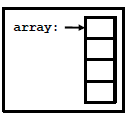
\includegraphics{sections/lec7/array.png}
	\end{center}
	\item If you were to look at the value of the variable ``array'' (not \lstinline[style=C++]{array[0]}) you'd find that it was exactly the same as the address of \lstinline[style=C++]{array[0]}.
	\item When the argument \lstinline[style=C++]{array} is passed to the function sum, a pointer to the first element of the array is really passed and the compiler does all the work of translating something like: \lstinline[style=C++]{array[3]} into the proper arithmetic/dereference to get the right value.
\begin{lstlisting}[style=C++]
x = array[3];
// Is equivalent to:
int *tmp;
tmp = array + 3;
x = *tmp;
// Or simply:
x = *(array + 3);
\end{lstlisting}
\end{itemize}

\subsection{Indexing vs. pointer arithmetic}
\begin{itemize}
	\item Using array indexing:
\begin{lstlisting}[style=C++]
for (int i = 0; i < SIZE; ++i){
	cout << array[i] << " ";
}
\end{lstlisting}
	\item Using pointer arithmetic:
\begin{lstlisting}[style=C++]
for (int *i = array; i < array+SIZE; ++i){
	cout << *i << " ";
}
\end{lstlisting}
\end{itemize}

\subsection{Array Traversal Using Pointers}
\begin{lstlisting}[style=C++]
int strlen(char *s) {
	char *p = s;
	while (*p) ++p;
	return p - s;
}
\end{lstlisting}
\begin{itemize}
	\item \lstinline[style=C++]{*p} evalues to ``false'' if \lstinline[style=C++]{p} points to a NULL, true otherwise.
	\item \lstinline[style=C++]{++p} advances by ``one character''
	\item \lstinline[style=C++]{p-s} computes the ``number of characters'' between \lstinline[style=C++]{p} and \lstinline[style=C++]{s}
\end{itemize}

\subsection{Constants}
\begin{itemize}
	\item \lstinline[style=C++]{void strcpy(char *dest, const char *src);}
	\item \lstinline[style=C++]{const} is a \textbf{type qualifier} - something that modifies a type
	\item It means ``you cannot change this value once you have initialized it.''
	\item When you have pointers, there are two things you might change:
	\begin{itemize}
		\item The value of the pointer.
		\item The value of the object to which the pointer points.
	\end{itemize}
	\item Either (or both) can be made unchangeable:
\begin{lstlisting}[style=C++]
const T *p;			// "T" (the pointed-to object) cannot be changed
T *const p;			// "p" (the pointer) cannot be changed
const T *const p;	// neither can be changed.
\end{lstlisting}
	\item Adding \lstinline[style=C++]{const} will stop changing value mistakes, and the compiler will catch them.
	\item You can use a pointer-to-T anywhere you expect a pointer-to-const-T, but NOT vice versa
	\item That's because code that expects a pointer-to-T might try to change the T, but this is illegal for a pointer-to-const-T.
	\item However, code that expects a pointer-to-const-T will work perfectly well for a pointer-to-T; it's just guaranteed not to try to change it.
\end{itemize}

\subsection{C strings vs. C++ strings}
\begin{center}
\begin{tabular}[breaklines=true]{p{5cm}|p{5cm}|p{5cm}}
	& C string & C++ string \\
	\hline
	Library headers & 
{\begin{lstlisting}[style=C++] 
#include <string>
\end{lstlisting}} & 
{\begin{lstlisting}[style=C++]
#include string
\end{lstlisting}}\\	
	string constant &
{\begin{lstlisting}[style=C++]
constchar* hello = "hello";
\end{lstlisting}}&
{\begin{lstlisting}[style=C++]
conststring hello = "hello";
\end{lstlisting}} \\
	length &
{\begin{lstlisting}[style=C++]
strlen(hello);//5
\end{lstlisting}} &
{\begin{lstlisting}[style=C++]
hello.length();//5
\end{lstlisting}} \\
	local variable &
{\begin{lstlisting}[style=C++]
constintMAXSIZE=1024; 
char s[MAXSIZE];
\end{lstlisting}} &
{\begin{lstlisting}[style=C++]
string s;
\end{lstlisting}} \\
	copy &
{\begin{lstlisting}[style=C++]
strcpy(s, hello);
\end{lstlisting}} &
{\begin{lstlisting}[style=C++]
s = hello;
\end{lstlisting}} \\
	concatenate &
{\begin{lstlisting}[style=C++]
constchar* world = " world";
char message[MAXSIZE];
strcpy(message, hello);
strcat(message, world);
\end{lstlisting}} &
{\begin{lstlisting}[style=C++]
string message = hello + " world";
\end{lstlisting}} \\
	compare &
{\begin{lstlisting}[style=C++]
if (strcmp(a,b) == 0)
	// do something
\end{lstlisting}} &
{\begin{lstlisting}[style=C++]
if (a == b)
	// do something
\end{lstlisting}} \\
	convert to C++ string &
{\begin{lstlisting}[style=C++]
string cpp_str = hello;
\end{lstlisting}} &
{\begin{lstlisting}[style=C++]
char c_str[MAXSIZE];
strcpy(c_str, message.c_str());
\end{lstlisting}} \\
\end{tabular}
\end{center}

\subsection{Type Sizes}
\begin{itemize}
	\item The amount of memory assigned to a data type is a source of innumerable ``portability bugs'' in programs.
	\item There are \textbf{some} guarantees, however:
	\begin{itemize}
		\item A ``char'' is always one byte
		\item A ``short'' is always at least as big as a char
		\item An ``int'' is always at least as big as a short
		\item A ``long'' is always at least as big as an int
	\end{itemize}
	\item \lstinline[style=C++]{sizeof(int)} tells you the number of bytes required to store an \lstinline[style=C++]{int}
	\begin{center}
		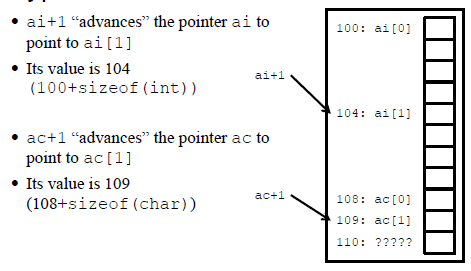
\includegraphics{sections/lec7/type.png}
	\end{center}
\end{itemize}

\section{More recurrent neural networks}

\section{Ways to make neural networks generalize better}

\section{Combining multiple neural networks to improve generalization}

\section{Hopfield nets and Boltzmann machines}
	\subsection{Hopfield Nets}
\begin{itemize}
	\item A hopfield net is composed of binary threshold units with recurrent connections between them
	\item Recurrent networks of non-linear units are generally very hard to analyze. THey can behave in many different ways:
	\begin{itemize}
		\item Settle to a stable state
		\item Oscillate
		\item Chaotic trajectories (cannot predict future)
	\end{itemize}

	\item John Hopfield realized that if the connections are symmetric, there is a global every function
	\begin{itemize}
		\item Each binary ``configuration'' of the whole network has an energy
		\item The binary threshold decision rule causes the network to a minimum of this energy function
	\end{itemize}

	\subsubsection{The energy function}
	\item The global energy is the sum of many contributions. Each contribution depends on one connection weight and the binary states of two neurons:
		$$E=-\sum_i s_i b_i - \sum_{i<j} s_i s_j w_{ij}$$
	\item This simple quadratic energy function makes it possible for each unit to compute locally how it's state affects the global energy:
		$$\text{Energy gap}=\delta E_i = E(s_i = 0) - E(s_i = 1) = b_i + \sum_j s_j w_{ij}$$
	\item Energy gap is the difference in energy when it is off minus when it is on
	
	\subsubsection{Settling to an energy minimum}
	\item To find an energy minimum in this net, start from a random state and then update units one at a time in random order
	\begin{itemize}
		\item Update each unit to whichever of its two states give the lowest global energy
		\item i.e., use binary threshold units
	\end{itemize}
	\begin{cetner}
		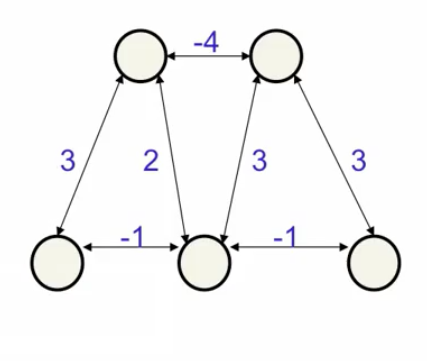
\includegraphics[scale=0.8]{sections/11/min.png}
	\end{cetner}
	$$-\text{Energy}=\text{goodness}=3$$

	\item A random unit is selected, and the question is asked: What state should that be in, given the current states of all other units?
	\begin{center}
		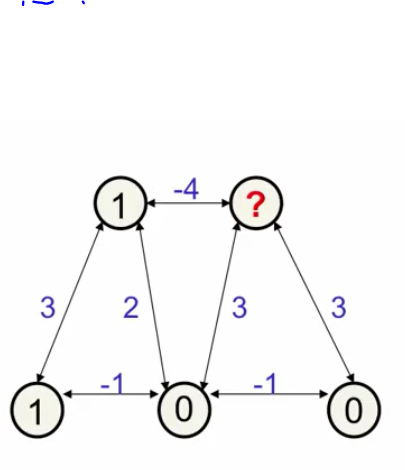
\includegraphics[scale=0.8]{sections/11/picked.png}
	\end{center}
	\begin{center}
		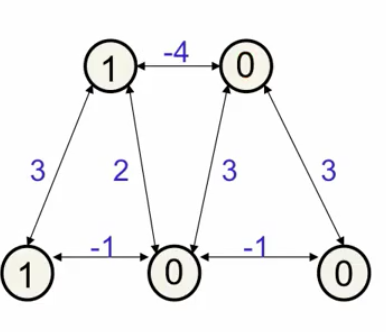
\includegraphics[scale=0.8]{sections/11/off.png}
	\end{center}

	$$-4(1)+3(0)+3(0)=-4<0\to \text{Turn off}$$
	\item Repeat for remaining units

	\subsubsection{A deeper energy minimum}
	\item The net has two triangles in which the three units mostly support each other
	\item Each triangle mostly hates the other triangle (-4 at the top)
	\item The triangle on the left differs from the one on the right by having a weight of 2 where the other one has a weight of 3
	\item So turning on the units in the triangle on the right gives the deepest minimum.
	\begin{center}
		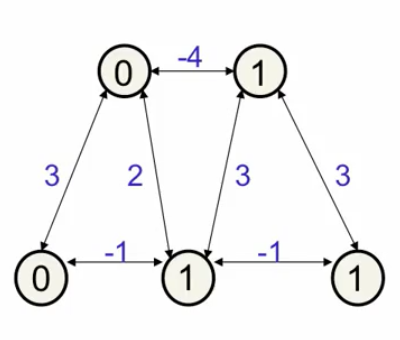
\includegraphics[scale=0.8]{sections/11/deep.png}
	\end{center}

	\subsubsection{Who do the decisions need to be sequential?}
	\item If units make simultaneous decisions the energy could go up
	\item With simultaneous parallel updating we can get oscillations
	\begin{itemize}
		\item Two units will continue to flip on and off
		\begin{center}
			\includgraphics[scale=0.9]{osc.png}
		\end{center}
		\item At the next parllel step, both units will turn on. This has very high energy, so then they will both turn off again.
	\end{itemize}

	\item If the updates occur in parallel but with random timing, the oscillations are usually destroyed
	
	\subsubsection{A neat way to make use of this type of computation}
	\item Hopfield proposed that memories could be energy minima of a neural net
	\begin{itemize}
		\item The binary threshold decision rule can then be used to ``clean up'' incomplete or corrupted memories
	\end{itemize}
	\item The idea of memories as energy minima was proposed by I.A. Richards in 1924 in ``Principles of Literary Criticism''
	\item Using energy minima to represent memories gives a content-adressable memory
	\begin{itemize}
		\item An item can be assessed by just knowing part of its content
		\item It is robust against hardware damage
		\item It's like reconstructing a dinosaur from a few bones
	\end{itemize}

	\subsubsection{Storing memories in a Hopfield net}
	\item If we use activities of 1 and -1, we can store a binary state vector by incrementing the weight between any two units by the product of their activities.
		$$\delta w_{ij} = s_i s_j$$
	\item This is a very simple rule that is not error-driven.That is both its strenght and its weakness. 
	\item We treat biases as weights from a permanently on unit
	\item With states of 0 and 1 the rule is slightly more complicated:
		$$\delta w_{ij} = 4(s_i - \frac{1}{2})(s_j - \frac{1}{2})$$
\end{itemize}

\section{Restricted Boltzmann machines (RBMs)}
	\subsection{Boltzmann machine learning}
\begin{itemize}
	\item Unsupervised learning problem
	\item We want the maximize the product of the probabilities that the Boltzmann machine assigns to the binary vectors in the training set
	\item Equivalent to maximizing the sum of the log probabilities that the Boltzmann machine assigns to the training vectors
	\item It is also equivalent to maximizing hte probability that we would obtain exactly the N training cases if we did the following:
	\begin{itemize}
		\item Let the network settle to its stationary distribution N different times with no external input
		\item Sample the visible vector once each time
	\end{itemize}

	\subsubsection{Why the learning could be difficult}
	\item Consider the chain of units:
	\begin{center}
		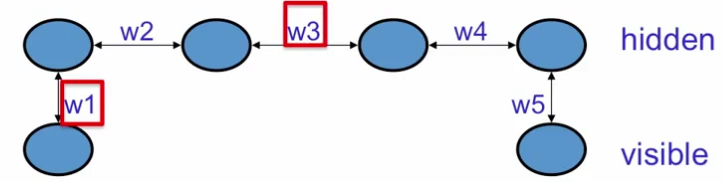
\includegraphics[scale=0.6]{sections/12/chain.png}
	\end{center}
	\item If the raining set consists of (1,0) and (0,1) we want the product of all the weights to be negative (So to know how to change w1 or w5 we must know w3)

	\item Everything that one weight needs to know about the other weights and the data is contained in the difference of two correlations:
	\begin{center}
		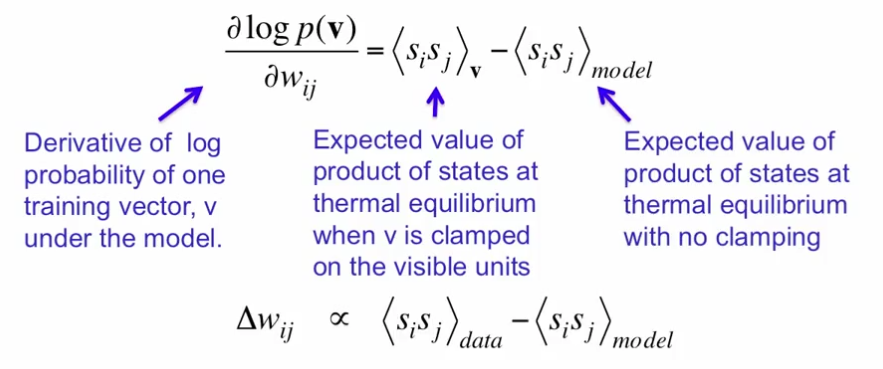
\includegraphics[scale=0.6]{sections/12/corr.png}
	\end{center}
		$$\delta w_{ij} \propto \langle s_i s_j \rangle_{data} - \langle s_i s_j \rangle_{model}$$

	\subsubsection{Why is the derivative so simple?}
	\item THe probability of a global configuration at thermal equilibrium is an exponential function of its energy
	\item So setting to equilibrium makes the log probability a linear function of the energy
	\item The energy is a linear fnuction of the weights and states, so:
		$$-\frac{\partial E}{\partial w_{ij}}=s_i s_j$$

	\item The process of settling to thermal equilibrium propagates information about the weights (We dontt need backprop)

	\subsubsection{Why do we need the negative phase?}
	\item Probability of a visible vector:
	\begin{center}
		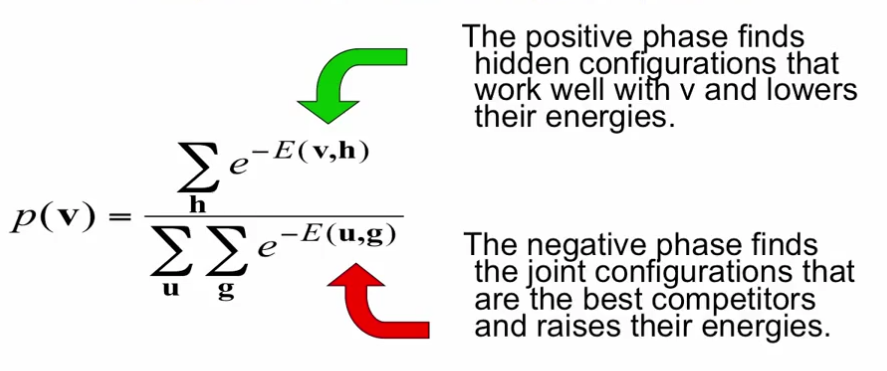
\includegraphics[scale=0.6]{sections/12/neg.png}
	\end{center}

	\subsubsection{An inefficient way to collect the statistics required for learning}
	\item \textbf{Positive phase}: clamp a data vector on the visible units and set the hidden units to random binary states
	\item Update the hidden units one at a time until the network reaches thermal equilibrium at a temperature of 1
	\item Once equilibrium, Sample $s_i s_j$ for every connected pair of units
	\item Repeat for al ldata vectors in the training set and average
	\item \textbf{Negative phase}: Set all the units to random states
	\item Update until equilibrium at temperature of 1
	\item Sample $s_i s_j$ for every connected pair of units
	\item Repeat many times and average to get good estimates
\end{itemize}

\section{Stacking RBMs to make Deep Belief Nets}

\section{Deep neural nets with generative pre-training}

\section{Modeling hierarchical structure with neural nets}

\section{Recent applications of deep neural nets}

\end{document}